% This document provides the style to be used for a MSc Thesis at the
% Parallel and Distributed Systems group
\documentclass[11pt,twoside,a4paper,openright]{report}

% math packages
\usepackage{amsmath}
\usepackage{amssymb}

% textblocks for title page
\usepackage[absolute]{textpos}

% use babel for proper hyphenation
\usepackage[british]{babel}

% Graphics: different for pdflatex or dvi output, choose one
%%\usepackage[dvips]{graphicx}
\usepackage[pdftex]{graphicx}
\usepackage{graphicx}

\usepackage{epstopdf}
\usepackage{rotating}
\usepackage{subcaption}

% FONT
\usepackage[scaled=.92]{helvet}
%\usepackage{times}
\usepackage{textcomp}

% for url's use "\url{http://www.google.com/}"
\usepackage{url}
\usepackage[plainpages=false]{hyperref} 

% Table
\usepackage{threeparttable, tablefootnote}
\usepackage{tabularx}

% References
\usepackage{flushend}


% Information that will be filled in at various points in the report
\newcommand{\reportTitle}{A Transiently-powered Battery-free Robot}
\newcommand{\reportAuthor}{Koen Schaper}
\newcommand{\reportEmail}{k.p.schaper@student.tudelft.nl}
\newcommand{\reportUrlEmail}{\href{mailto:\reportEmail}{\reportEmail}}
\newcommand{\reportMSC}{Embedded Systems} %{Embedded Systems}{Computer Engineering}{Computer Science}{Electrical Engineering}
\newcommand{\reportDate}{\today} %TODO: Dit is de datum van uitgifte van final versie aan de afstudeer commissie 
\newcommand{\presentationDate}{\today} %TODO: Dit is de datum van de afstudeerpresentatie 
\newcommand{\graduationCommittee}{
prof. dr. K.G. Langendoen (chair) & Delft University of Technology \\
dr. Przemys\l{}aw Pawe\l{}czak (supervisor) & Delft University of Technology \\
} % The order of listing the names: Graduation prof, supervisor(s), others ordered by title + alphabetical 
%examples: 
%prof. dr. ir. H. J. Sips (chair) & Delft University of Technology \\ 
%ir. dr. D. H. J. Epema           & Delft University of Technology \\ 
\newcommand{\reportAbstract}{TODO ABSTRACT}
\newcommand{\reportKeywords}{TODO KEYWORDS}

% For pdflatex
\pdfinfo{
   /Author (\reportAuthor)
   /Title  (\reportTitle)
   /Keywords (\reportKeywords)
}

\begin{document}

\pagenumbering{alph}
\pagestyle{empty}


% FRONTCOVER
%%\usepackage[total={210mm,297mm},left=0pt,bottom=0pt,top=0cm,right=0pt,headsep=0pt,head=0pt,showframe]{geometry}

%%\input{preambleL31958}
%%\begin{titlepage}
\begin {textblock*}{210mm}(0mm,0mm)
\noindent

\includegraphics[height=3.2cm]{pics/block}
\sffamily
\vspace{.8cm}
\begin{center}
\Large
Delft University of Technology\\
Master's Thesis in \reportMSC\\
\vspace{2cm}
\parbox{170mm}{\bfseries\centering\Huge\reportTitle}\\
\vspace{1cm}
\parbox{170mm}{\bfseries\centering\reportAuthor}

\end{center}
\end{textblock*}


\begin {textblock*}{210mm}[0.0,1.0](0mm,297mm)
\noindent

\hfill\parbox{15.5cm}{
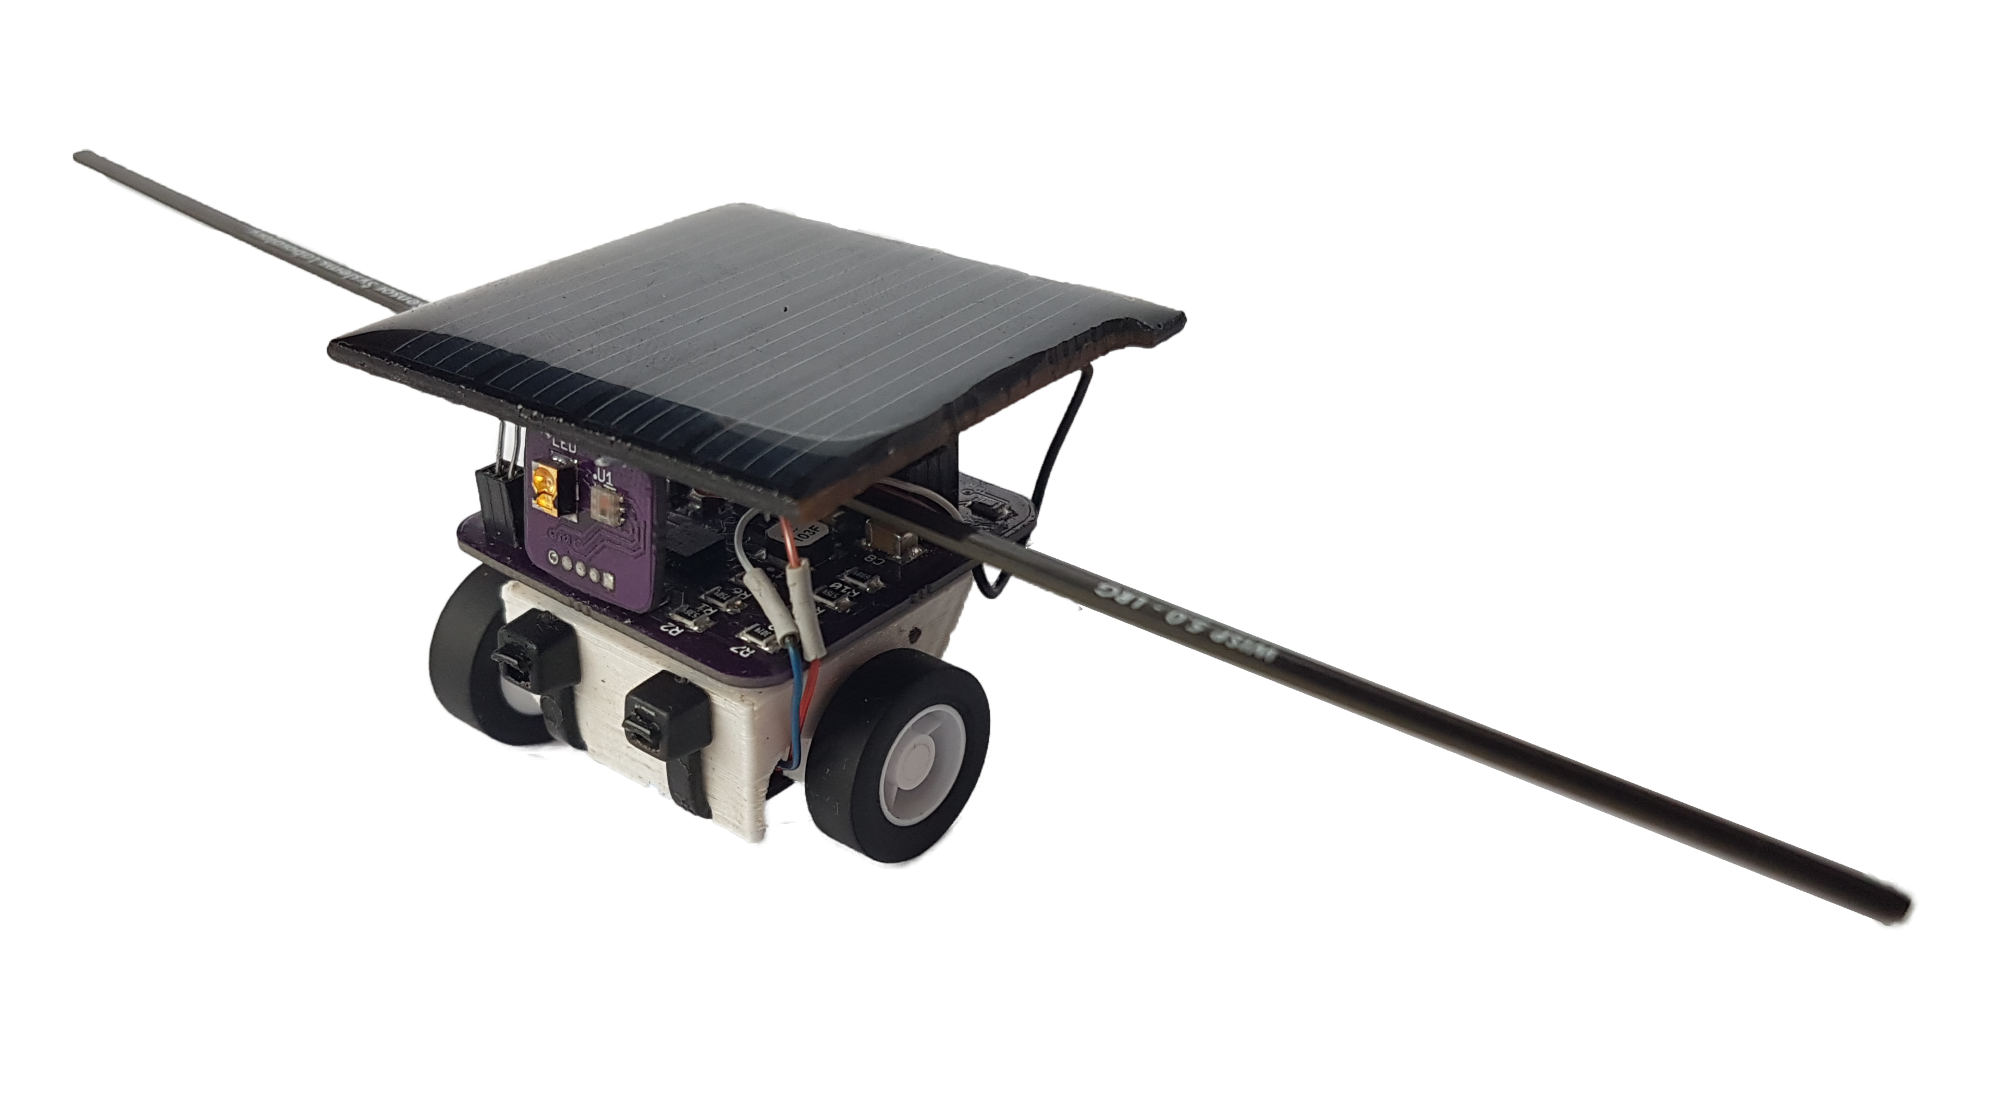
\includegraphics[width=13cm]{pics/tp_robot.png}
}
\vspace*{4cm}

\noindent
\hspace{1.89cm}
\hfill\parbox{5cm}{

\includegraphics[width=5cm]{pics/es_logo_cyan_black_rgb}}
\hspace*{2cm}\\

\vspace*{1.5cm}
\noindent

\includegraphics[width=\textwidth]{pics/TU_border_A4_L_front}
\end{textblock*}

\null\newpage


%%%%%%%%%%%%%%%%%%%%%%%%%%%%%%%%%%%%%%%%%%%%%%%%%%%%%%%%%%%%%%%%%%%%%%%%%%%%%%%
\hoffset=1.63cm
\oddsidemargin=0in
\evensidemargin=0in
\textwidth=5in

%%%%%%%%%%%%%%%%%%%%%%%%%%%%%%%%%%%%%%%%%%%%%%%%%%%%%%%%%%%%%%%%%%%%%%%%%%%%%%%
\parindent=1em

% EMPTY PAGE
\cleardoublepage

\pagestyle{plain}
\pagenumbering{roman}
\setcounter{page}{1}

% TITLE PAGE: page i (hidden)
\begin{titlepage}

  \begin{center}
  \null\vfill
    \begin{center}
    \LARGE{\reportTitle}
    \end{center}

    \vspace{3cm}

    \begin{large}
    Master's Thesis in \reportMSC
    \end{large}

    \vspace{1.5cm}

    \begin{normalsize}
    Embedded Software Section\\
    Faculty of Electrical Engineering, Mathematics and Computer Science\\
    Delft University of Technology\\
    Mekelweg 4, 2628 CD Delft, The Netherlands
    \end{normalsize}

    \vspace{2.0cm}

    \begin{normalsize}
    \reportAuthor \\
    \reportUrlEmail
    \end{normalsize}

    \vspace{1.0cm}

    % <MM> DD, YYYY
    \reportDate             %TODO: Dit is de datum van uitgifte van final versie aan de afstudeer commissie

  \vfill
  \end{center}

\end{titlepage}


% GRADUATION DATA AND ABSTRACT: pages ii and iii (hidden)
%De aankondiging bevat de spreker, titel, plaats, datum en tijd, samenstelling van de afstudeercommissie en een korte samenvatting (maximaal 25 regels).
\thispagestyle{empty}

\noindent \textbf{Author}\\
\begin{tabular}{l}
\reportAuthor{} (\reportUrlEmail)\\
\end{tabular}\\
\noindent \textbf{Title}\\
\begin{tabular}{l}
\reportTitle\\
\end{tabular}\\
\noindent \textbf{MSc presentation}\\
\begin{tabular}{l}
% <MM> DD, YYYY (like \today)
\presentationDate\\
\end{tabular}

\vspace{1.1cm}

\noindent \textbf{Graduation Committee}\\
\begin{tabular}{ll}
\graduationCommittee
\end{tabular}


\begin{abstract} %de abstract bevat alleen een korte samenvatting van de inhoud van het onderzoek
\setcounter{page}{3}
\reportAbstract{}
\end{abstract}

\clearpage

%\setcounter{page}{4}

% EMPTY PAGE: page iv
\cleardoublepage

% OPTIONAL QUOTATION: page v
%\pagestyle{empty}

\null\vfill

\begin{center}
\emph{``TODO QUOTE''} -- TODO QUOTED PERSON
\end{center}

\vspace{10cm}

\clearpage


% EMPTY PAGE: page vi
%\cleardoublepage

% PREFACE: page v
\chapter*{Preface}
\addcontentsline{toc}{chapter}{Preface}

This thesis presents the final work done towards obtaining my master’s degree in Embedded Systems from Delft University of Technology.
To the best of my knowledge no previous work has been conducted, exploring the feasibility of a transiently-powered battery-free robot. 


\vspace{1\baselineskip}

\noindent
I would like to express my sincere gratitude to my supervisor Przemys\l{}aw Pawe\l{}czak for his excellent guidance, never failing support and enthusiasm about this project. 
I also would like to thank Amjad Majid for letting me explore his idea of transiently-powered actuation, his constructive criticism and clever suggestions as this project evolved.
Moreover, I would like to thank Sinan Yildirim for his willingness to answer any of my questions, Ioannis Protonotarios for helping me with any hardware related issues, Michel Jansen for sharing his schematics.
Additionally, I would like to thank the Nuon Solar Team for lending me one of their space grade solar panels from their 2017 Nuna9 solar car.
Furthermore, I want to thank Prof. Koen Langendoen for hosting me at the Embedded Systems group, and Javier Alonso-Mora for participating as a member of my graduation committee.
Last but not least, a special thanks to my family for their unconditional support, encouragements and love that helped me stay motivated during this year.

\vspace{1\baselineskip}

\noindent
Koen Schaper

\vspace{1\baselineskip}

\noindent
Delft, The Netherlands

\noindent
\today

% EMPTY PAGE: page vi
\cleardoublepage

% TABLE OF CONTENTS: starting at page vii
\tableofcontents

\cleardoublepage

\pagenumbering{arabic}
\setcounter{page}{1}

% INTRODUCTION: page 1
\chapter{Introduction}
\label{chp:introduction}

% printer: Tethered flight control of a small quadrotor robot for stippling \cite{galea_iros_2017}

% Estabish your territory

Miniature robots with limited capabilities can work together in "swarms" to achieve more than an individual could by itself, but are still far from being applicable in real world applications~\cite{barca_sekercioglu_2013}.
The future potential of swarms is widely recognized to have applications in surveillance, search and rescue, and exploration.
Swarms have been proposed as a new form of user interface, robots can display information and interact with users on tabletops~\cite{legoc_uist_2016}, unmodified clothing~\cite{dementyev_uist_2016} and can be an educational toy for kids~\cite{sony_toio_2017}.
\hfill \break

% Establish nice
% Motivation for this work: Why do we want to remove the battery?

However, one of the fundamental issues that needs to be addressed before swarm robotics can advance is related to energy, small lithium batteries are currently powering the robots and limit their operation time to only a view hours. 
The energy density of batteries has improved less than 1 order of magnitude since 1945, in comparison the energy efficiency of computing has improved 12 orders of magnitude~\cite{patel_pvc_2017}.
The last major advancement in battery technology is 25 years old and came with the introduction of Li-ion batteries.
Additionally, any new big improvements in energy density of batteries is not likely to happen anytime soon, as new battery technologies are often overhyped and slow to emerge~\cite{zachary_spec_2016}.
\hfill \break

%TODO introduce current research

% Propose a solution: Energy harvesting
% And discuss current solutions to autonomus operation / battery replenishment

A stable energy supply is a current requirement to allow long term persistent autonomous operation of swarm robots.
Relaxing this constraint by allowing a transient supply of energy could be a potent area of research.
Wireless sensor nodes that rely on energy harvesting have already been emerging, some are highly energy constrained but fully eliminate the need for batteries.
In contrary, different replenishment methods for robot batteries are currently used, robots can be moved to a charging station leaving them nonoperational while recharging or the battery could be replaced, resulting in a high strain on maintenance.

% 4 lines left!
\newpage

\section{Problem statement}

% What why how

% Intermittently powered robots, that purely rely on harvested power are currently non existent.

Replacing a robots battery with an energy harvesting system could make it more self sufficient and energy-autonomous. 
This however introduces a new phenomenon to take into account; the intermittent availability of energy produces frequent power interrupts.
The possibility of sudden power loss is currently not considered when developing software that controls a robots behavior, and for this reason can not be used without adaption.
\hfill \break

Secondly, sensors and control techniques used may not be found applicable due to energy budget constrains or their inability to be interrupted by a loss of power. 
Different locomotion types are used and may not all be reliable and/or accurate under the frequent power interruption.
This research will explore the feasibility of a miniature battery-less robot, allowing persistent operation while being supplied with a small and intermittent source of energy.
Therefore the main question this work will try to answer is:

\begin{center}
	\textit{How to enable a transiently powered robot to operate autonomously?}
\end{center}

\section{Contributions}
Current swarm robots assume that a task can only be completed if sufficient energy is left in the batteries, which also limits their operation time. 
While surprisingly this is the first study of transiently powered robots, unaware of any platforms being implemented and are operating under the constant threat of power loss. 

\begin{enumerate}

%\item A simple model is developed showing the relation between the energy stored, weight of the robot, frequency of power cycles and distance covered with a single charge.

\item Design of a battery-less robot that purely operates from harvested energy, with basic capabilities allowing autonomous operation.

\item Implementation of a control algorithm, that allows the robot to finish a movement across power cycles.

%\item Evaluation of the battery-less robot compared to a battery powered robot in terms of, weight, speed and accuracy of movement.


\end{enumerate}


\section{Thesis Outline}
%What will be discussed in the coming chapters


\vspace{1\baselineskip}

\noindent
TODO ORGANISATIONAL DESCRIPTION OF THESIS



% CHAPTERS ... For instance: History/Prior Work, Design/Implementation, Experiments
\chapter{Related Work}
\label{chp:related_work}

This chapter will provide background information about current state of the art transiently powered systems. The advantages and disadvantages of different electrical storage types are compared. A short summary of current miniature robotics platforms is given and commonly used locomotion types. Finally different methods that try to ensure continuous operation will be discussed.

\section{Transiently-powered systems}
\label{sec:tp_systems}

% - Roughly everything that is powered fron a Energy harvester

Example of energy harvesting: Prolonged energy harvesting for ingestible devices~\cite{plonski_tranro_2016}
Drug delivery
\\
Converting a Plant to a Battery and Wireless Sensor with Scatter Radio and Ultra-Low Cost

%Other sources available for exploration are often limited by the application. Secondly, most sources can be scarce or completely absent during prolonged time intervals of the day as well \cite{RN15}. 

Fully programmable RFID platforms have been developed to exploring the combination of sensing, computation and communication, while allowing battery-less operation by harvesting RF energy~\cite{sample_transim_2008}.
The amount of energy collected from RF signals is very small and decreases with the distance of the device to the transmitter.
The harvested energy is typically stored in a capacitor, where larger capacitors can buffer more energy and smaller capacitors have the advantage of shorter charge times~\cite{gummerson_mobisys_2010}.
For longer, complex operations the energy budged needs to be evaluated carefully.
To store the energy an appropriate size storage capacitor needs to be selected~\cite{naderiparizi_rfid_2015}.

% - Short intro into persistent framwork: checkpointing etc
% mementos
% chain
% ratchet

\section{Energy Supply}
\label{sec:energy_supply}

% Explain battery vs supercapacitor

Comparing li-ion batteries with super-capacitors there are some big differences.
Supercapacitors do not need any special charging scheme and circuity for charging, except for overcharging protection.
Secondly, super-capacitors do not require any particular current profile, the energy can be stored at any rate and when the energy is required it can be extracted at any power level.
Operating a li-ion battery outside of it's recommended operating conditions can severely reduce a batteries lifetime and result in overheating or even explosion of the battery.
Batteries will seldom withstand more than one thousand complete charge/discharge cycles.
Super-capacitors used under extreme condition's, are not likely to explode but instead rupture.
While the biggest disadvantages of super-capacitors is their low energy density and high price, their lifetime is typically hundred thousands of charge/discharge cycles.

Li-Ion Battery-Supercapacitor Hybrid Storage System for a Long Lifetime, Photovoltaic-Based Wireless Sensor Network	\cite{ongaro_pwre_2012}
Reincarnation in the Ambiance: Devices and Networks with Energy Harvesting \cite{prasad_comst_2014}



\section{Small robotic platforms}
\label{sec:robotic_platforms}

%TODO tell that these robots are used for studing swarm behavior (inspired by nature)
% require communication to apply different algorithms
% need to be low cost and size are key factors for allowing scalability
% 
%Main characteristics : https://link.springer.com/article/10.1007/s11721-012-0075-2
%robots are autonomous;
%robots are situated in the environment and can act to modify it;
%robots’ sensing and communication capabilities are local;
%robots do not have access to centralized control and/or to global knowledge;
%robots cooperate to tackle a given task.

Low cost robotic platforms have been developed to tackle a variety of challenges anonymously.
Miniature robots can be used for inspection in difficult to reach places, operating like mobile sensing units.
Hardware modularity is a way to make the robot adapt its resources to different environments and sensing operations.
By separating out power, computation, motor control and sensing a verity of capabilities can be tested~\cite{sabelhaus_icra_2013, pickem_icra_2015, kim_iros_2016}.
Microrobots typically use infrared-based neighbor to neighbor distance sensing and communication~\cite{rubenstein_icra_2012, pickem_icra_2015, kim_iros_2016}.
While controlling a swarm or collective is mainly accomplished by means of active low power transceivers~\cite{sabelhaus_icra_2013, pickem_icra_2015, kim_iros_2016}. 

%TODO reference table

\section{Locomotion}
\label{sec:locomotion}
%TODO tell somthing about their accuracy!

Choosing the right locomotion resource can depend on different factors, moving in the most energy efficient way on a particular surface is often the determining factor.
On a flat surface, robots commonly use a two-wheeled differential drive design to not only move but allow for steering as well~\cite{sabelhaus_icra_2013, pickem_icra_2015}.
The GRITSBot does not use conventional DC motors, requiring encoders to estimate their speed. 
Instead by using stepper motors the speed can be set by changing the delay between steps. 
Estimating it's position therefore is reduced to simply counting steps~\cite{pickem_icra_2015}.  
Overall cost can be a decisive factor, therefore the Kilobot uses two vibrating motors for locomotion combined with three thin legs.
When the motors are activated the centripetal forces will generate a forward movement, which can be explained using the slip-stick principle~\cite{rubenstein_icra_2012}.
Other locomotion types are biologically inspired, the HARM-VP is small scale piezoelectric driven quadrupled robot~\cite{baisch_iros_2013}.
Each leg as two degrees of freedom, it can move up and down, as well as forward and backward.

\section{Continuous operation}
\label{sec:continous_operation}
%Battery replenishment

%TODO include battery tosti iron anecdote
Typically the operation time is extended by regularly checking the remaining energy in the battery and move to a recharging station before the robot runs out of energy~\cite{pickem_icra_2015, rubenstein_icra_2012}.
As an alternative to quickly recharging, the battery can also be swapped automatically when the robot moves into the docking station~\cite{kemal_mech_2015}.
Another work shows a robot which is able to swap it's primary battery using a six degree-of-freedom manipulator, used to grab the dead battery and plug it into a wireless recharging charging station \cite{zhang_conel_2013}.
Using direct wireless power to replace or supplement to a batteries energy is shown in~\cite{karpelson_icra_2014}, however the robot can only operate or recharge while remaining in close proximity to a transmitter. 
In these cases the robots are highly reliant on an infrastructure to allow for continuous autonomous operation.
This can be a severe constraint if the robot moves out of reach or needs to operate in a area where this infrastructure is not present. Persistent operation can also be achieved by harvesting renewable energy, particularly solar energy to complement to the robots internal energy source. To remove weight from the robot, in \cite{bruhwiler_iros_2015} the solar energy is used directly without any type of energy buffer. A drawback of this method is that the incoming solar energy should already greater or equal to the energy required for operation. This approach has been tested for basic locomotion and did not combine any form of sensing and control.

% - Provide overview table robots smaller than 15*15cm

% For each of these cases you need to provide numbers: 
% level of autonomy (does the robot does all by itself or relies on external processing)
% does autonomy fall under 
% charging time

% Add missing "new" robots

\begin{table*}[t]
	\centering
	\tiny
	\begin{threeparttable}
		\caption{An comparison of small robotic platforms}
		\label{tab:comparison_robot_platforms}
 		\begin{tabularx}{\textwidth}{l l X X X l l l} 
			\hline
 			Robot & Cost & Scalability & Sensors & Locomotion & Size [cm] & Weight [g] & Battery life \\ 
 			\hline
 			IPR & TBD & charge, program & gyro, distance, ambient light & wheel, 25cm/s & 4.0 & 21 & 1s\\
 			HAMR-VP\textsuperscript{1} \cite{bruhwiler_iros_2015} & NS & none & gyroscope, optical mouse & legged, 1cm/s & 4.4 & 2.3 & 3m \\
 			Roverables \cite{dementyev_uist_2016} & NS & charge & wheel, distance, optical encoders & wheel, ?? & 4.0 & ?? & 45m \\ 
 			Zooids \cite{legoc_uist_2016} & \$50 & ?? & position, touch & wheel, 50cm/s & 2.6 & 12 & 1-2h \\ 
 			mROBerTO \cite{kim_iros_2016} & \$60\textsuperscript{1} & program & light, range, gyro, camera, accel., compass, distance, bearing & motor shaft, 15cm/s & 1.5 & ?? & 1.5h\\
 			GRITSBot \cite{pickem_icra_2015} & \$50\textsuperscript{2} & charge, program, calibrate & distance, bearing, 3d accel., 3d gyro & wheel, 25cm/s & 3 & ?? & 1-5h \\
 			Kilobot \cite{rubenstein_icra_2012} & \$50\textsuperscript{2} & charge, program & distance, ambient light & vibration, 1cm/s & 3.3 & ?? & 3-24h\\
 			TinyTerp \cite{sabelhaus_icra_2013} & \$50 & none & 3d gyro, 3d accel. & wheel, 50cm/s & 1.8 & ?? & 1h\\
			\hline
		\end{tabularx}
		\begin{tablenotes}
			\item [1] Modified to include on-board power, sensing and control.
			\item [2] Cost of parts
		\end{tablenotes}
	\end{threeparttable}
\end{table*}

\chapter{Robot Design and Implementation}

% - Size and weight/energy availability/speed trade-off model and 
% - Should the subsections more or less reflect the columns in the table?
% - No optical encoders because they require a lot of energy!
% - Same for linefolower / mouse sensor.

\section{Design Requirements}
\label{sec:design_requirements}

% - Small form factor
% - Navigation
% - Power (should not rely on batteries)
% - However should be able to be powered from batteries for testing and tuning!
% - Tradeoff chargetime and operation time
% - Weight of the robot
% - Low voltage decreases power consumption of components and allows efficient use of the energy from the supercapacitor
% - Single mainboard design
% - Swarm robots are typically limited to only operate on flat surfaces!
% - Limited resources (no power hungry components ie optical encoders or mouse sensors)
% - Optimize or low power consumption (disable or standby sensors and motor ctrl when not used)

% RF harvesting seems prommesing
% Wispcam requires approx 4 seconds to harvest 20mJ at a distance of 20cm from the reader \cite{naderiparizi_rfid_2015}
% better to only use RF for communication and harvest energy from another source \cite{konstantioulos}

% Why rf: low power transmitter requires a lot of power (maybe datasheet ref??)


The main requirement for the robot is  that it should be battery-less, therefore it can only store a small amount of energy in a capacitor / small buffer.
Bigger capacitors have in general larger leakage currents.
As a result these require longer charge time

Size of the robot i.e weight and the required power for movement do not scale linearly.

To make efficient use of the energy stored in a supercapacitor a regular is required to supply a stable voltage to the connected loads.
The regulated output voltage is a lower threshold for the energy that can be used from the capacitor.
The upper threshold is typically determined by the maximum voltage rating of the supercapacitor.
Lowering the output voltage allows for more energy to be used from the supercapacitor, but also lowers the overall power consumption of individual components.
The energy stored in supercapacitor is a function of the capacitance and the threshold voltage difference, being equal to:

\begin{equation}
\label{eq:cap2}
E = \frac{1}{2}C(V_{max} - V_{min})^{2}
\end{equation}


	
\section{Hardware Implementation}

% - EXPLAIN MORE ABOUT HARDWARE CHOISES, why these specific componens. What were the requirements for choosing these components

The first step was to evaluate what components are required for the robot to have basic navigation capabilities.
Based on this, there was searched for commercially available low power components with the lowest minimal supply voltage.
Currently there are only a limited amount of motor controllers on the market that can operate at the 2.0V.
To make sure that a small drop in system voltage would not create instability a margin of 0.2V was added.
Now the system voltage of 2.2V has been determined, each part of the robot will be explained in more detail. 

\subsection{Computation and Sensing}

The robot is designed around a WISP 5 \cite{wisp5_wiki_2017}, a battery-free platform for low power sensing, computation and communication.
This platform has the ability to communicate with RFID readers and is powered by the carrier signal emitted by the reader.
However, the communication range and the power that can be harvested is limited.
Therefore communication is currently not implemented and a different energy source for harvesting will be used.
Currently only the microcontroller is being utilized, a Texas Instruments MSP430FR5969 ultra low power microcontroller.
This MCU can operate at 16 MHz and features 64 KB FRAM, 2 KB SRAM and 40 IO.

The robot has access to basic sensors which can be interfaced trough I2C.
For detecting obstacles in front of the robot, a Maxim Integrated MAX44000 proximity sensor was added of the robot facing forward.
This sensor switches a IR led at high frequency to reduce the power consumed.
The same sensor is based around a photo-diode it can be used to measure the amount of ambient light as well.
To allow for controlled movements the robot has a Bosch Sensortec BMG250 low power triaxial gyroscope to measure yaw-rate, used to correct it's heading when necessary.

\subsection{Locomotion}

% tell that also higher geared motors were tried??

Two dc motors with a 25:1 gearbox from Precision Microdrives are mounted in a 3d printed frame. %, directly under the mainboard of the IPR.
The motors are mounted diagonally opposite from each other making the robot as compact as possible, while this differential drive configuration allows the robot to steer.
Small plastic wheels with rubber tires are mounted directly on each of the motor shafts.
Behind these two motors a free running caster wheel is mounted to the frame, acting as a third support point for the robot.

The speed of each motor can be controlled individually using Pulse-Width-Modulation (PWM) and a Texas Instruments DRV8836 dual H-bridge.
Typically MCU io-ports are limited in the amount of current that they can supply.
MOSFETs inside the dual H-bridge allow regulation of larger currents to the motors.
The MCU can use the H-bridge to enable, disable and control the direction of rotation of each individual motor.

%TODO tell something about the maximum speed that can be achieved

On average the each motor consumes 38mA while running on a flat surface, which is well within the current limit that the buck converter can supply.
However when the motors are in not moving yet the start current is approximately equal to the stall current, which is equal to 240mA.
This amount of current can not be supplied by a most regulators, PWM can be used to reduce the average current allowing a bulk capacitor to supply the voltage.

\subsection{Energy Harvesting}
\label{subsec:energy_harvesting}

Solar energy is harvested from two IXYS SLMD121H04L-ND solar cells in series.
These monocrystalline solar cells have a high efficiency of 22\%, allowing energy harvesting even in low light conditions.
The solar cells are connected to a Texas Instruments BQ25570 energy harvester. 
This harvester includes a nanopower boost charger with maximum power point tracking to extract the optimal amount of energy from the solar panel. 
The harvested energy is stored in a 22mF - 4.5V supercapacitor from AVX, chosen for it's low leakage current and small size.
The Texas Instruments BQ25570 has a buck converter to efficiently regulate the capacitor voltage down to the system voltage of 2.2V.
External resistors can be used to program voltage thresholds, allowing to automatically enable and disable the buck converter based on minimum and maximum thresholds.
Additionally the resistors are used to set the overvoltage protection and the buck converter output voltage.

\subsection{Integration}

A complete overview of the robot can be found in Figure \ref{fig:robot_overview}.
Most components are part of the Printed Circuit Board (PCB), only the larger components are mounted externally.

% Tell why pcb is required.
% Low power compontents have chip packages which are hard to solder by hand because of their small package size.
% More stability
% Tell about the Printed Circuit Board(PCB)

Now that all the parts have been chosen, they can be connected together to form the robot.
For ease of connection and because the ICs come in small no-leads packages, a PCB has been designed, see Figure \ref{fig:pcb_robot}
Most reference designs are extendable but this adds complexity, while weight and size are the main constraints of this robot design.



\begin{figure}
	\centering
	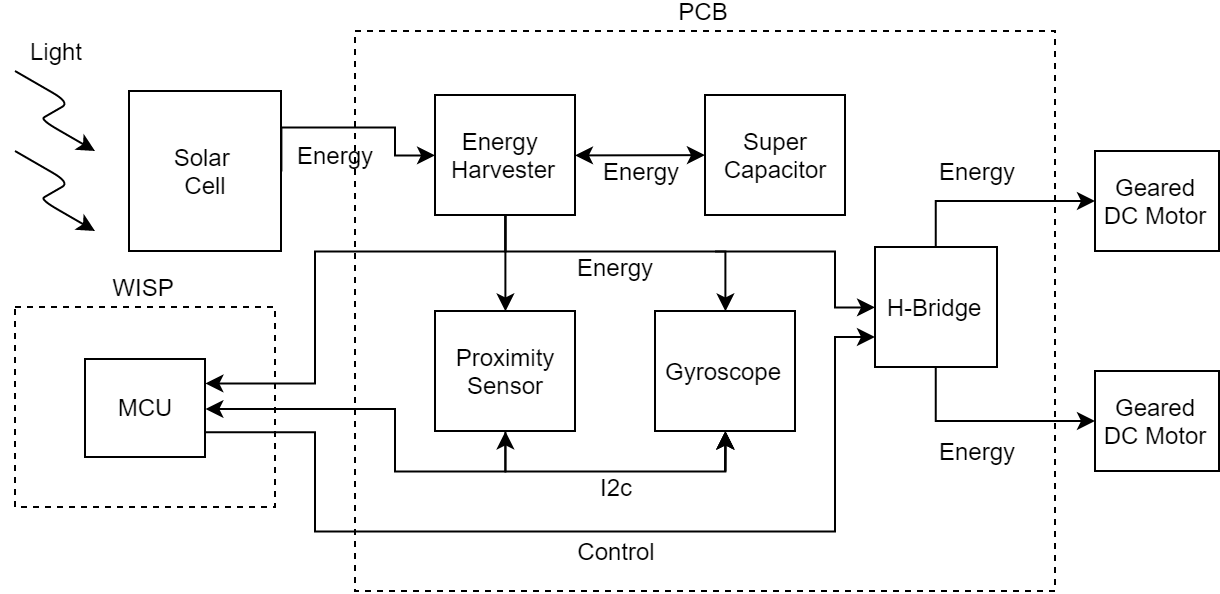
\includegraphics[width=\textwidth]{pics/schematic_robot_v2.png}
	\caption{Overview of a single robot}
	\label{fig:robot_overview}
\end{figure}


\begin{figure}
	\centering
	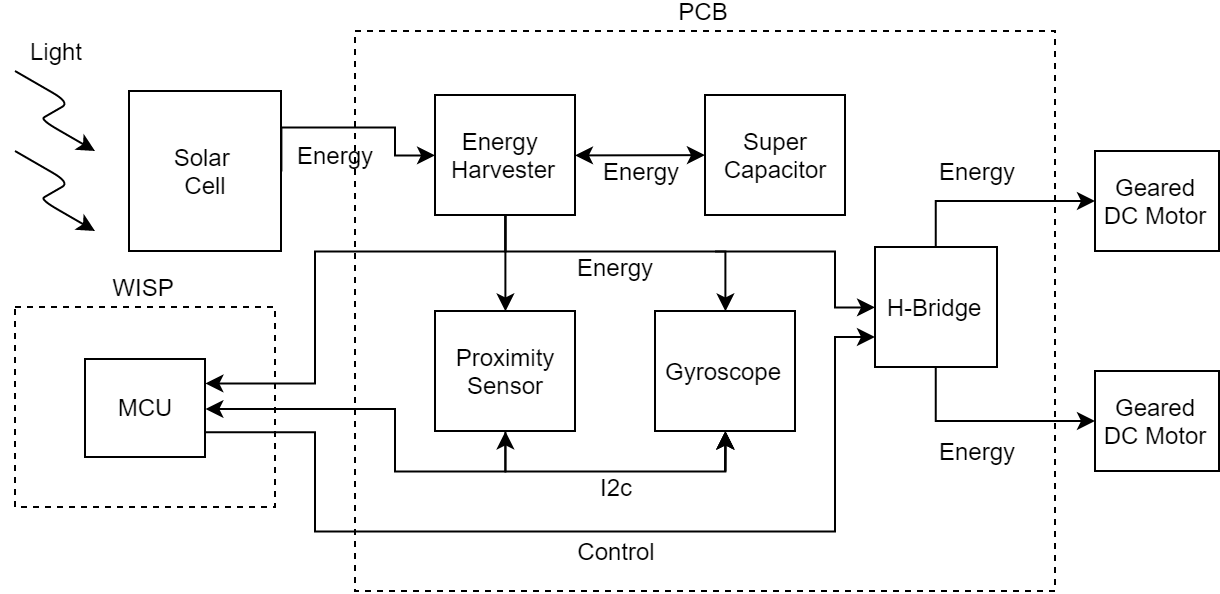
\includegraphics[width=\textwidth]{pics/schematic_robot_v2.png}
	\caption{PCB DESIGN}
	\label{fig:pcb_robot}
\end{figure}


% Make a overview of the cost to build a robot

\begin{table*}[t]
	\centering
	\caption{Power consumption of each individual component at 2.2V}
	\label{tab:1}
	\begin{tabular}{l l l} 
		\hline
		\\[-1em]
		Part & Active Current & Standby Current\\ 
		\hline
		\\[-1em]
		Proximity sensor & 432\textmu A & 0.1\textmu A \\
		Gyroscope & 650\textmu A & 3\textmu A\\	
		Microcontroller @ 8MHz & 1mA & N/A \\
		H-bridge & 1.2mA & 10nA \\
		DC motor & 39mA & N/A \\
		DC motor & 39mA & N/A \\
		\hline
		\\[-1em]
		Total & xx & xx \\
	\end{tabular}
\end{table*}


\section{Software Implementation}

% General library for reading and writing to i2c.

% How program consistency (ie progress) is maintained given the intermittend nature of the robot.

% A operating system for intermittend devices

\subsection{Calibration of the motors}
\label{subsub:motor_calib}

% Write about why valid to assume a constant speed on a single surface
In robotics the motors are commonly powered directly from the battery as linear or switch-mode power regulators are not able to supply the high start-up currents.
When the motors are powered from the battery the supplied voltages drops while energy is consumed for the battery.
Since the speed of the motor is dependent on the supply voltage the speed of the motor will also decrease while energy is consumed from the battery.
However, the use of a supercapacitor requires a regulator to make efficient use of the energy stored, as described in Section \ref{subsec:energy_harvesting}.
A benefit of running a constant voltage is that the supply voltage is not a factor anymore which can change the motor speed.
NEED MORE EXPLANATION
By making the assumption that the robot will only travel on a flat surface, the speed is considered constant given a certain PWM duty-cycle.


\subsubsection{PWM frequency for linear motion control}
% Write about linear motion control dc motor vs pwm
% Reference: https://www.precisionmicrodrives.com/application-notes/ab-022-pwm-frequency-for-linear-motion-control

Pulse width modulation(PWM) is used to control the speed of the motors, by changing the duty cycle of the control pulse the average current through the motors can be changed.
The winding current is proportional to the torgue output of the motor and therefore the average winding current is proportional to the PWM duty cycle.
However this is only true for pure resistive loads,

%Typically operation frequency is above 20 khz (what people can hear)

% -Write how the pwm control signals are generated for the H-bridge. 
The PWM signals are generated by the microcontroller on the WISP.
Luckily four io-ports are available on the WISP which can be directly controlled by a single timer running at 2kHz.
The timer is configured to use a compare register for each of the ports.
When the timer reaches a value that corresponds to a value one of the compare registers the connected port is toggled automatically.
This way the overhead is minimized because no interrupt service routine is required.

\subsubsection{Duty cycle selection}

The next step is to determine the minimum and maximum PWM duty-cycle that will enable the motor to turn.
A minimal PWM duty-cycle to produce a torque that is able to overcome the static friction between the wheels and a surface the robot is moving on.
Each motor is physically different and the friction in the gearbox can variate as well, which results in a different output speed per motor.
Since the robot uses two motors in differential drive configuration, a minimum PWM duty-cycle has to be found for each motor.
This is accomplished by setting a PWM duty-cycle at which both motors are rotating and slowly backing down the PWM duty-cycle until one or both stop turning.
The minimum PWM duty-cycle, allowing the wheels to rotate, is then saved and added to every motor set point.
If the robot is commanded to run at this minimum speed it will be very likely that it will not yet travel in a straight line.

% -Write about maximum speed due to enabling two motors and their startup current peak! show figure!!
% -Write about current generated by the lack of Back-EMF
% -Use large capacitor to somewhat reduce the effect! NEED FIGURE!
%TODO -Write about bounding the pid output, because otherwise the motors of the robot could stall, if the motor setpoint is to high
% Does more gearing (more torque) reduce the current peak??
% How does pwm influcence the startup current of the motor in combination with a capacitor
% The pwm frequency seems to have a effect as well; higher freq preforms better??
% Maybe something with RC TIME?

The maximum PWM duty-cycle is bounded by the amount of current that the buck converter and bulk capacitor can supply.
Lowering the PWM duty-cycle can reduce the current peak induced by the lack of back-EMF when the motor is in steady state.
When the set point is just to high a kind of clicking noise can be heard, indicating that the start current peak of motor is to high and the power supply is not able to supply the current.


\begin{equation}
\frac{dV}{dt} = \frac{I}{C}
\end{equation}

Allow 0.2V voltage drop (msp430 and motor driver stop working)

% DO calculation of current that can be supplied from capacitor buffer

 


\subsection{Closed loop feedback for controlled movements}

The robot uses two physically different motors in differential drive configuration which are mounted in a non-symmetrical way.
Open loop movement using just a calibrated motor values has been used in previous work \cite{legoc_uist_2016}, but it can be time consuming and any little disturbance will trow the robot off course.
The gyroscope is used to obtain the current yaw-rate and correct the robots heading.
Controlled movements are possible using closed loop feedback, where the heading is used to update the motor control values.

The robot can be controlled using three different commands, one for straight trajectories, one for left and one for right turns.
When a command is executed a control loop will run until the provided target is reached.
A timer running periodically calling a interrupt service routine which executes the control loop.   
Each command requires different initial values, set points and tuning parameters, these are set accordingly before the control loop is enabled.

\subsubsection{Controlled straight trajectories}

% -Why pid for straight movements and not a simple p controller?
% --Fast reaction on disturbances without osccilation??

The control loop for straight trajectories obtains the yaw-rate from the gyroscope and uses this as an input for the Proportional–Integral–Derivative (PID) controller.
The PID will try to reduce the error and force the yaw-rate to zero for a given target motor speed.
% $ e(t) = 0 - yaw(t)$
Using the output of the PID controller the target motor speed of each motor is adjusted in opposite direction.
The loop will stop automatically when the required target is reached.
%TODO Explain that the target distance is with a calibrated value.

\begin{equation}
output(t) = K_{p}e(t) + K_{i} \int_{0}^{t}e(\tau)d\tau + Kd\frac{d}{dt}e(t) [rad/s]
\end{equation}

\subsubsection{PID tuning using Ziegler-Nichols method}

%TODO -Write about tuning the pid controller using Ziegler–Nichols tuning method (method 2), closed loop, Critical gain.

A PID loop can be tuned using three different tunable gains ($K_{p}$, $K_{i}$, $K_{d}$).
Tuning can be done trough a trail and error approach but a faster way of tuning is to use the Zigeler-Nicholos method.
The second or ultimate gain method starts with increasing or decreasing Kp until constant oscillation occurs.
From Figure \ref{fig:ultimate_gain} can be seen how the proportional gain was increased until eventually the robot started to oscillate.
With a proportional gain of 0.13 the robot starts light oscillation at the end, but this is not always the case and can be a result of the surface the robot was driving on.
% Tell something about how the right values are determined
To reduce the oscillation a $T_{u}$ of 0.2 was added as can be determined from Figure \ref{fig:gain_tuning}.
From this figure can be seen that the robot is more stable and doesn't have the intension to oscillate anymore.
Robots was driving on surface that was not super flat, therefore the gyro signal is noisy.
The tuning process was sped up by setting the minimum motor duty-cycle as it made the robot a lot more responsive, this was described earlier in Section \ref{subsub:motor_calib}.

%TODO -Add figure with critcial gain + mark period Tu

\begin{figure}[!tbp]
	\begin{subfigure}[b]{0.5\textwidth}
		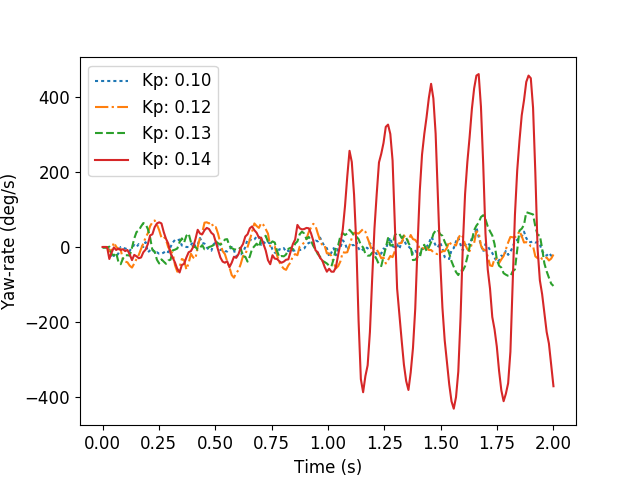
\includegraphics[width=\textwidth]{pics/straight_ku.png}
		\caption{Increase Ku until oscillation}
		\label{fig:ultimate_gain}
	\end{subfigure}
	\begin{subfigure}[b]{0.5\textwidth}
		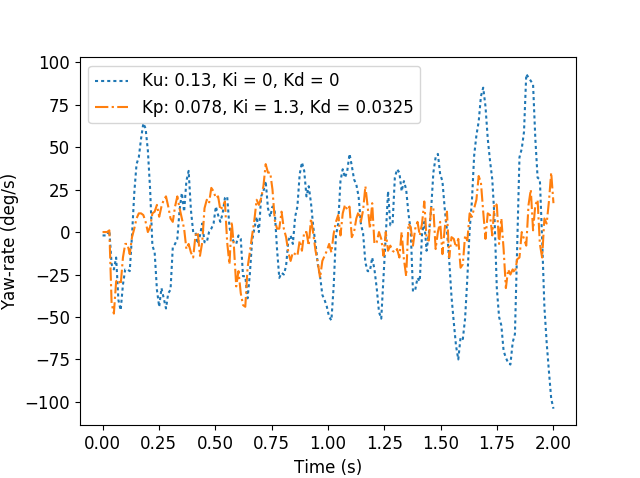
\includegraphics[width=\textwidth]{pics/straight_ku_with_tu.png}
		\caption{Find period}
		\label{fig:gain_tuning}
	\end{subfigure}
	\caption{Tuning the PID controller using the ultimate gain method}
\end{figure}

\subsubsection{Controlled turns}

The control loop for controlled turning uses the angle, which can be obtained by integrating the yaw-rate sensor data from the gyroscope.
A P controller is used to rotate the robot to the desired angle, the proportional gain is directly influencing turn speed of the robot.
The motor control values are set to run the motors opposite directions and are equal to the output of the P controller.
These values will keep decreasing until the robot rotates to the desired angle.
The set point is assumed to be reached when the angle is within two degrees of the target, in this case the loop will stop automatically.
To allow enough precision to be able to measure if the target is within these two degrees, the timer which executes the control loop was set to run at 100Hz.
Secondly, the proportional gain should not be set to low because it can happen that the robot is not able to reach the target but also not to high as it can overshoot the target.

\subsection{Persistent movement}

% Checkpointing / State keeping

% Dubble buffering for updating multiple dependent variables (keep consistency)

\chapter{Evaluation} 

% - Weight vs current consumption vs distance
% - Measure start motor overhead and average consumption (show graph?)


\section{Performance in different light conditions}
% Casestudy of conditions robot 
% outdoors/indoors/varying light sources/varying solar panels
% Do experiment in sunlight for nuna panel

%The amount of energy that can be harvested from normal office lighting is limited.
Currently the robot harvests energy form light using a small solar panel.
However, there isn't always enough sunlight available to charge the robots in a acceptable time.
To allow the robots to have sub ten second charge times, a lighting setup needs to be created that provides a reasonable amount of uniform light to the area where the robots move around.
In this section the charge time of the supercapacitor is evaluated, while it's charged from different solar panels and different light sources.

\subsection{Experimental setup}
% Temperature and Light intensity?
To accurately measure the power that is harvested from each solar panel all the experiments were preformed in a darkroom.
The setup consists of a light source that can be positioned at multiple distances from a solar panel.
The solar panel is connected to input of the harvester on the PCB of the robot and when the voltage in the supercapacitor reaches the threshold the buck converter of the energy harvester is enabled.
Voltage is supplied to the WISP which is programed to only enable a GPIO port and enable a LED.
A Saleae Logic, logic analyzer is connected to the port and used to record the time required to charge the capacitor from the minimum to the maximum value.
The port is enabled the light source is disabled and the LED is used to drain the energy from the capacitor.
When the led turns off, indicating that a new charge period begins, the light source is enabled again.
Now a more detailed description will be given of the different components that were tested.

%TODO Why these lamps?
Three different solar panels were tested in this experiment. Information about the solar panels can be found in Table \ref{tab:solar_panels}.
Low cost solar simulators can consist of a combination of LED and halogen light bulbs to simulate sunlight and are used to test the performance of solar panels~\cite{grandi_tia_2014}.
However, in this case the goal is to have a controlled uniform lighting environment where the robots have roughly constant charge times.
Solar panels do not only harvest energy from the visual light spectrum but harvest almost at least as much from the infrared light spectrum, therefore not only light but also heat will shorten the charge time.
Halogen lamps have a lower color temperature than the sun but also emit waves far into the infrared spectrum.
The light sources used in this experiment are a 60W halogen bulb, a 120W halogen halogen bulb and two 150w IR heat lamps where one is colored red.
Three measurements were done, where the lamps were positioned 10cm, 30cm and 50cm from the solar panels.
Additionally, for these three distance the temperature was measured at the solar panel using a K-type thermocouple supplied with an Extech EX330 multimeter and the light intensity using the luxmeter on a MASTECH MS8229 multimeter.

\begin{table}[t]
	\centering
	\begin{threeparttable}
		\caption{The solar panels tested in the experiment}
		\label{tab:solar_panels}
		\small
		\begin{tabular}{|l|l|l|l|}
			\hline
			& Composition & Efficiency & Dimensions \\
			\hline \hline
			Banggood \cite{bangood_solar_2017}& Poly-Si & 17\% & 40x30mm \\
			\hline
			INYS SLMD121H04L-ND\textsuperscript{1}& Mono-Si & 22\% & 43x34mm \\
			\hline
			Azurspace 3G28C & Triple Junction GaAs& 28\% & 80x40mm \\
			\hline
		\end{tabular}
	\begin{tablenotes}
		\small
		\item [1] Two panels in parallel
	\end{tablenotes}
	\end{threeparttable}
\end{table}

\subsection{Results}
% No difference between the heatlamps in power consumed
% Halogen distributes the light more even
% Panel from nuna
% Refer to appendix for temperature and light data?

Both the temperature and illumination increase by decreasing the distance between the light source and the solar panel. 
Secondly, increasing the output power of the lamp increases temperature and illumination as well. 
However the charge times 
A thing to note is that the both the 60w and 150w ir lamps have a spherical design. This creates a uneven circular shadowing pattern on the surface the lamps are shining on, which becomes more significant on the bigger distances in this experiment.
The 120w lamp has a tubular design and in combination with the light fixture most of the light is reflected down with minimal shadowing of the lamp resulting in a more even light distribution.

\begin{figure}
	\centering
	\begin{subfigure}[b]{0.49\textwidth}
		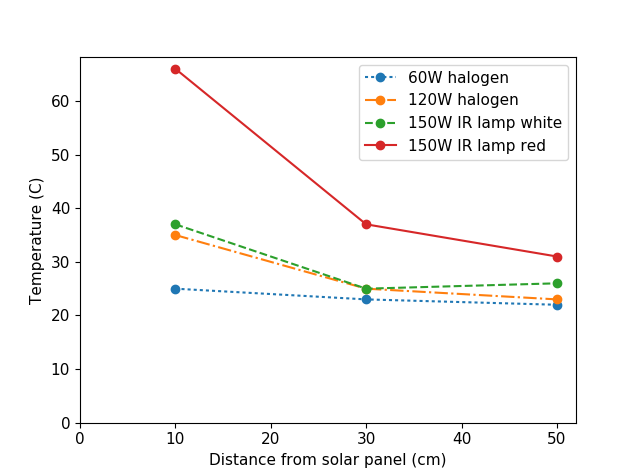
\includegraphics[width=\textwidth]{pics/light_experiment_temp.png}
		\caption{Temperature at different distances}
		\label{fig:light_temp}
	\end{subfigure}
	\begin{subfigure}[b]{0.49\textwidth}
		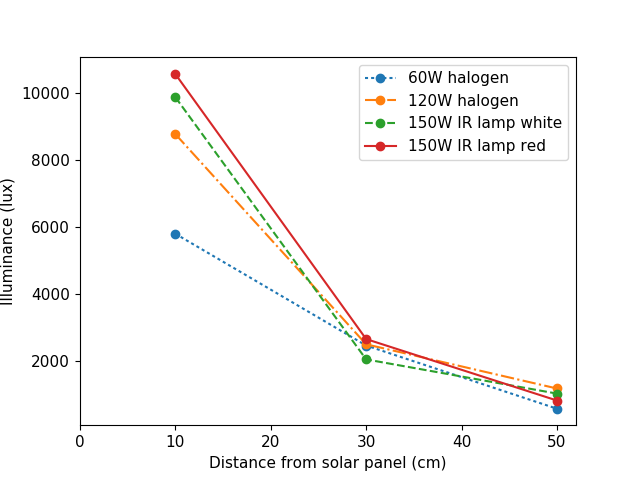
\includegraphics[width=\textwidth]{pics/light_experiment_lux.png}
		\caption{Light intensity at different distances}
		\label{fig:light_lux}
	\end{subfigure}
	\caption{}
\end{figure}


\begin{figure}
	\centering
	\begin{subfigure}[b]{0.49\textwidth}
		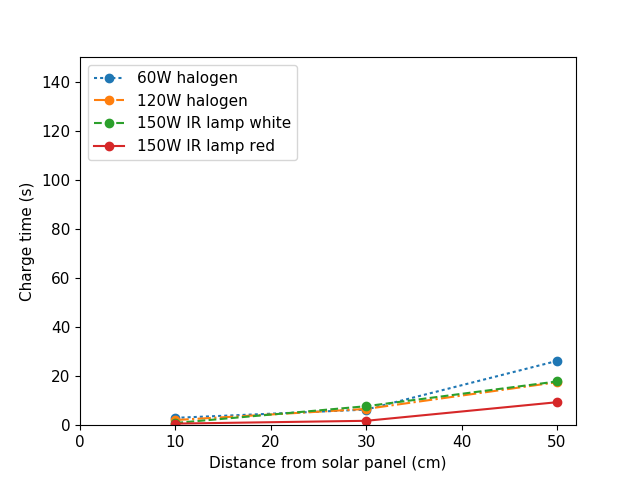
\includegraphics[width=\textwidth]{pics/light_experiment_figure1.png}
		\caption{Ebay panel}
		\label{fig:light_exp1}
	\end{subfigure}
	\begin{subfigure}[b]{0.49\textwidth}
		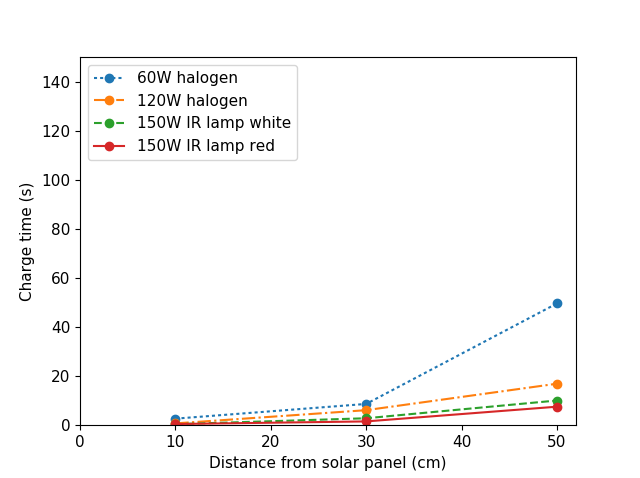
\includegraphics[width=\textwidth]{pics/light_experiment_figure2.png}
		\caption{IXYS SLMD121H04L-ND}
		\label{fig:light_exp2}
	\end{subfigure}
	\begin{subfigure}[b]{0.49\textwidth}
		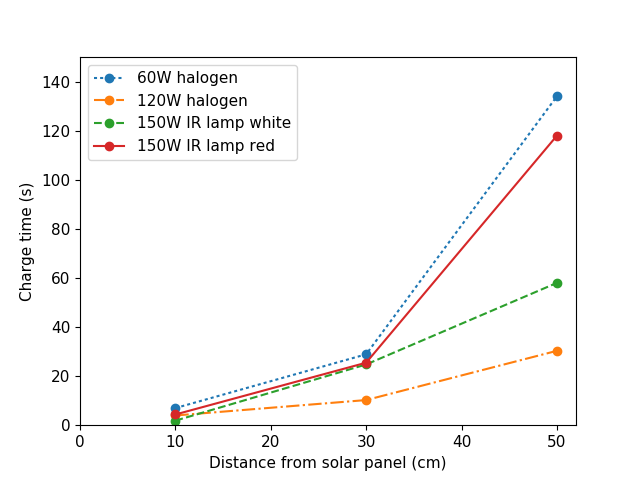
\includegraphics[width=\textwidth]{pics/light_experiment_figure3.png}
		\caption{Azurspace 3G28C}
		\label{fig:light_exp3}
	\end{subfigure}
	\caption{The performance of three different solar panels for different distances from different light sources. The data charge times for the last two are normalized with respect to the surface covered by the first panel.}
\end{figure}


\section{Controlled Movements}
\label{sec:controlled_movements}

% Comparison deadreckoning accuracy of battery powered robot with solar powered robot

% Try at least one more supercapacitor: 10mF
% Study reducing the frequency of power interrupts ie smaller energy buffer.
% How does this effect the accuracy of locomotion?

% Study the effect of checkpoint frequency on the straight and turn accuracy + combination
% Before and after counting in case of current robot

% Video of robot movement

Now that a variety of solar panel / light combinations has been evaluated, the next Section will evaluate the accuracy of movement of the robot and will compare the battery-less robot and it' battery powered equal.

\subsection{Experimental setup}

To be able to compare the accuracy of the robot while it is exposed to increasingly smaller power cycles, a variety of movements is recorded using a overhead camera.
A camera stand with DSLR camera is positioned on a tabletop and in the camera's view the corners of a square of 80 x 80 cm are indicated with a black marker, see Figure \ref{fig:movement_setup}.
This square can later be used as a reference to convert the robots movement from pixels to cm.

Three different movements are compared, while the robot is moving straight movement of 75 cm, a circle with radius of 30cm and a square of 50 by 50 cm.

\subsubsection{Artificial Power Interrupts}

%TODO Why bat powered
During the experiment the robot will be powered from a battery and power interrupts, i.e the capacitor running out of energy are created artificially using a timer that resets the MCU.
The MSP430FR5969 has the functionality to enable a brownout reset trough software which is used to simulate the event of the supply voltage dropping below the required operating voltage.
With a capacitor of 22mF the robot can operate around 1 second, this resulted in the chosen interrupt periods.
Choosing a period smaller than half a second resulted in uncontrolled behavior, while the control loop was not able to stabilize the movement before the robot runs out of energy again.
Therefore the power interrupt periods evaluated in this experiment are: 1.25, 1, 0.75 and 0.5 seconds.

\subsubsection{Velocity calibration}

%TODO make table with standard deviation of distance traveled 
Each movement is executed at three different PWM target settings: 40\%, 65\% and 90\% of the maximum duty cycle.
To let the robot move a particular distance, the average speed needs to be estimated for each PWM target and power interrupt period.
This is achieved by first determining the time that the robot requires to move approximately 150 cm for each target without power interrupts.
When the robot experiences power interrupts the average velocity of a active period becomes lower due to frequent acceleration from standstill.
With power interrupts the runtime is increased to make the robot travel roughly the same distance.
Finally, the average of five measurements is computed and divided by the commanded runtime of the robot to acquire an average speed for each combination.


\subsubsection{Tracking the robots Movement}

A robot is programmed to preform the movement at a desired velocity and optional power interrupt period.
Before the robot executes the movement a green led is enabled on top of the robot, this bright green dot will be the reference point that the tracking software will try to follow.
The camera is used to record the movement which is analyzed using Python and OpenCV 3.2, a example of a tracked movement can be seen in Figure \ref{fig:movement_example}.

\begin{figure}
	\centering
	\begin{subfigure}[b]{0.45\textwidth}
		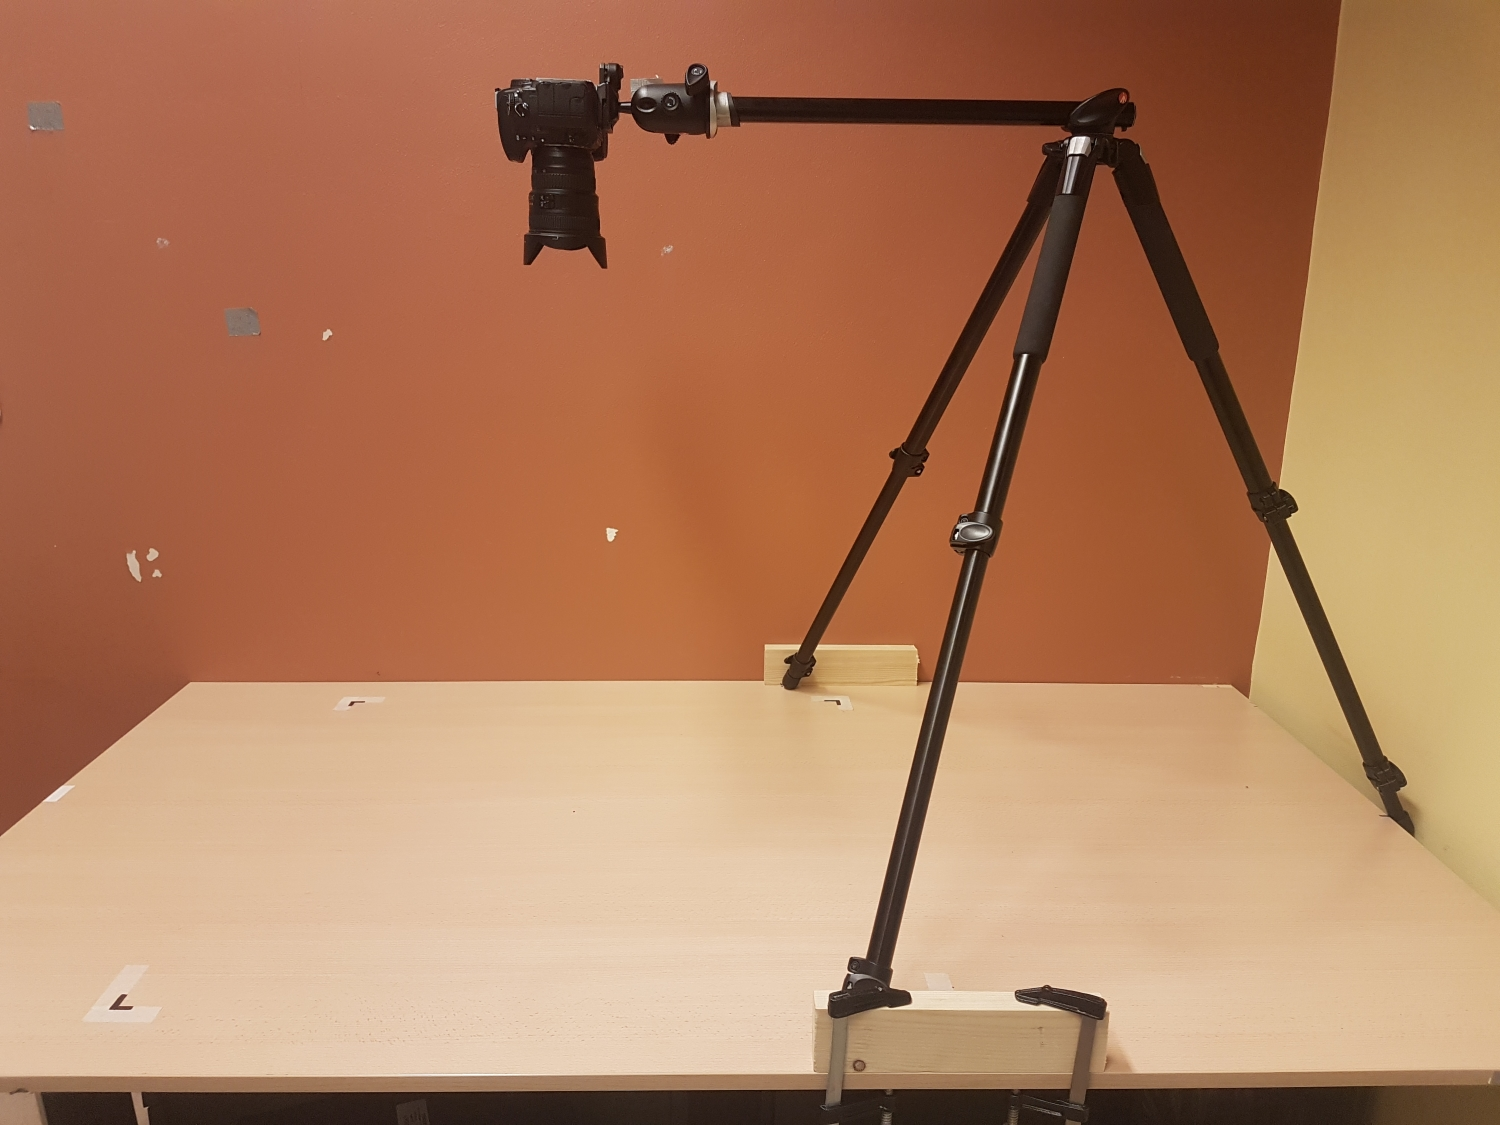
\includegraphics[width=\textwidth]{pics/movement_setup.jpg}
		\caption{Camera setup}
		\label{fig:movement_setup}
	\end{subfigure}
	\quad
	\begin{subfigure}[b]{0.45\textwidth}
		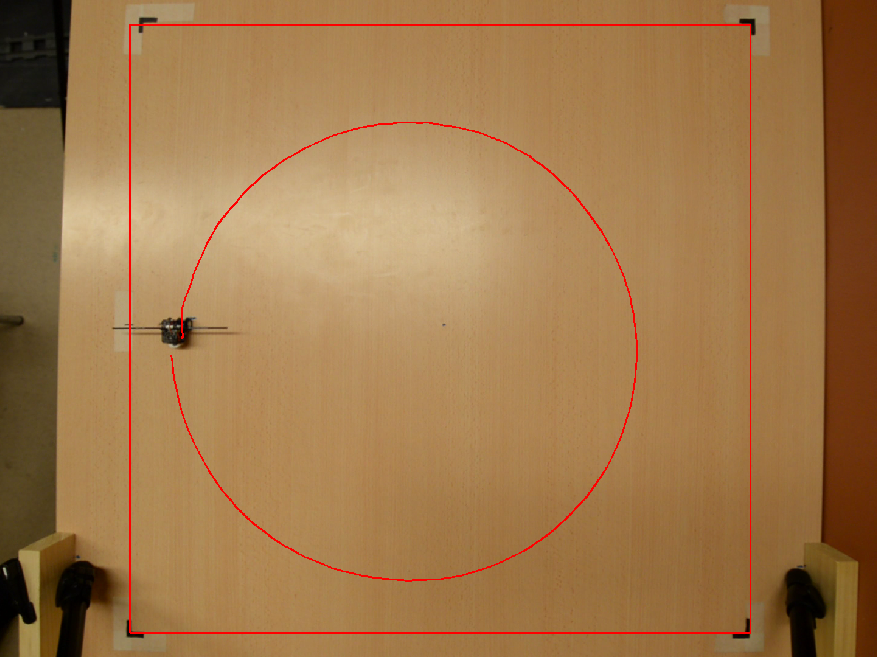
\includegraphics[width=\textwidth]{pics/movement_example.png}
		\caption{Tracking with OpenCV}
		\label{fig:movement_example}
	\end{subfigure}
	\caption{Recording the robots movement}
\end{figure}


\subsection{Movement Accuracy Metrics}

for straight movements: the amount of curvature

standard deviation in length of movement for each type of movement

\subsection{Straight Movements}




\subsection{Curved Movements and Turns}


\subsection{Results}

Hoe de interrupts uitkomen op de beweging heeft invloed!!

Lager snelheid en minder interrupts is hogere precisie??




% CONCLUSIONS AND FUTURE WORK
\chapter{Summary}
\label{chp:summary}

%This thesis is surmised by a conclusion in Section \ref{sec:conclusion} and in Section \ref{sec:limitations_future_work} possibilities for future work will be presented.

\section{Conclusion}
\label{sec:conclusion}

In this thesis, a transiently-powered robot is designed and implemented that uses light as a source of energy.
Two geared dc motors have been chosen to provide locomotion to the robot and their startup current peak is limited using PWM.
A controller is designed that allows for controlled straight and curved movements, while a simple check pointing method combined with persistent movement targets allows a movement to be completed across multiple power cycles.
Multiple movements have been executed and recorded using an overhead camera.
Tracking software is used to verify the accuracy of a transiently-powered battery-free robot and compares it performance to a battery powered equivalent robot.
By decreasing the interrupt period, a lower threshold of 0.3\,s has been found in which case the robot started to show uncontrolled behavior, i.e. significant drift to the side of the weakest motor.
The amount of time that power is available might not be sufficient for the motors to reach their steady state speed, making controlled movements using linear motor control impossible.
Using artificial power interrupts, the results show that decreasing the interrupt period towards the lower threshold results in increased horizontal deviation in case of straight movements.
This is suspected to be caused by more frequent accelerations from standstill.
For curved movements the results show a decreased average deviation from the fitted circle by increasing the target duty cycle.
The additional speed is suspected to allow the controller to be more effective in steering the robot towards its final destination.
The solar powered robot surprisingly outperforms the battery-powered robot in terms of movement accuracy, as the additional weight of the solar panel is suspected to have a positive effect on the movement of the robot.

%Section \ref{sec:controlled_movements} shows that the transiently powered robot is able to execute an instructed motion with similar accuracy compared to a battery powered equal. 
%The distance covered by a robot with frequent power interrupts in a certain amount of time is smaller, i.e the average speed is lower due to frequent acceleration from a standstill.

\section{Future Work}
\label{sec:limitations_future_work}

The capabilities of the current robot can easily be extended by using more features from the WISP or by designing a custom alternative.
Additional features that could be implemented in future work are:

\begin{itemize}

\item \textbf{Speed feedback}: 
In order to move a certain distance with a higher accuracy, an energy efficient speed feedback method is required.
One option is to add local speed sensing or another option is to supply external position feedback to the robot.

%One option could be to determine motor speed by measuring the Back-EMF produced by the motor, as it is proportional to the motors revolutions per minute~\cite{precision_backemf_2017}.
%Another method could use wheel encoders without an active light source and instead use ambient light, already available in abundance because it is used as the source of energy.

\item \textbf{Lack of communication}: 
Communication with an external host is not implemented.
The energy efficient backscatter communication channel of the WISP could be used.
Even though power cycles will occur less frequent when compared to the RFID, due to relative large supercapacitor, they still pose a challenge in externally controlling the robot.

\item \textbf{Transiently-powered swarm}: 
With a communication channel, a new promising area of research is to create a swarm of transiently powered robots.
The effect of intermittentcy on the behavior and controllability of this type of swarm needs to be investigated.
This research could further investigate the portability of existing swarm algorithms or propose new solutions.	

\item \textbf{Size reduction}: 
In order to further reduce the weight of a robot there is a need to move away from DC-motors, since significant smaller and efficient DC-motors are not available.
%Alternative legged locomotion types have been discussed in Section \ref{sec:rw_locomotion}.
Miniature legged robots that make use of piezoelectric actuators seem promising, but most of them are still in an early stage of development.

\item \textbf{Sensing capabilities}: 
Future applications may require additional sensors to be added to the robot to extend its capabilities.
However, the power consumption, frequency of use and the accuracy trade off needs to be evaluated carefully since the energy budget is limited.


\end{itemize}

%\item \textbf{TP swarm OS} 
%Recently, embedded operating systems~\cite{trenkwalder_iros_2016} and extendable programming~\cite{pinciroli_iros_2016} languages have been created to speed up the development process of swarms, removing the need to focus on low level interactions and individual behaviors.
%In addition, multiple task and checkpoint based methods have been developed to enable computation across power cycles as described in Section \ref{sec:comp_pc}.
%Merging both paradigms could help to speed up development of transiently powered swarms. 



%\subsection{Path planning based on energy availability}

%To capture the optimal amount of solar energy along the way, a map of the expected solar power can be used to compute the optimal path. To distinguish sunny or shaded two methods are proposed in \cite{plonski_tranro_2016}, one being a simple data driven Gaussian Process and the other estimates the geometry of the environment as a latent variable.
%Energy aware path planning is commonly used in combination with mission planning.
%In \cite{kaplan_iros_2016}, an analysis of the solar radiation is used to generate a time-optimized motion plan and power schedule using a cascaded particle swarm optimization algorithm.
%By combining maps of lighting and ground slope a solar-powered robot can be kept illuminated continuously. A connected component analysis is used to plan a optimal route on traversable slopes, as described by \cite{otten_icra_2015}.

% BIBLIOGRAPHY
%#define SORTED 1
%\bibliographystyle{../bib/latex8}
%\bibliography{../bib/bibtex}

\bibliographystyle{IEEEtran}
\bibliography{IEEEabrv,bib/bibtex}

%\appendix

%\chapter{TODO APPENDIX NAME}
\label{app:}
Appendix body



\end{document}

